\section{System Overview}
\label{sec:volumetric:system_overview}
Figure~\ref{fig:volumetric:proposedCandidate} shows an overview of our NED's hardware and operation. Our proposed display consists of three main active optical components namely: (1) an HDR Illuminator, (2) a DMD chip, and (3) a focus-tunable lens. These three optical components are driven at high-speed by an FPGA, a microcontroller, and custom electronics. 

The focus-tunable lens is driven in a continuous mode such that its optical power follows a triangular or sinusoidal waveform. The DMD projector is synchronized with the focus-tunable lens to display a stack of binary frames in each lens cycle, and the HDR illuminator illuminates the DMD chip with a distinct selected RGB color for each binary frame. Each cycle of the focus-tunable lens is one frame of the overall display. To avoid confusion, each frame of the DMD will be referred to as \emph{single-color binary image} whereas the 24-bit color rendering of the 3-D scene will be referred to as the color image.

Our DMD's refresh rate is $f_{\text{DMD}} = 16,800$ Hz, and our target display refresh rate is $f_{\text{NED}}=60$ Hz. Then the number of single-color binary images displayed by the DMD in each frametime of the NED is given by
\begin{equation}
N_b = \frac{f_{\text{DMD}}}{f_{\text{NED}}} = 280.
\label{eq:280}
\end{equation}

These $280$ single-color binary images are distributed in depth along the user's line-of-sight from 15cm to 4M.  Correct modeling of the depth distribution and field-of-view (FoV) of binary images is necessary for proper rendering and color decomposition. 

The optical design of our NED is discussed in Section~\ref{sec:volumetric:Optical_design} and the rendering pipeline that converts 3-D scene information into multiple single-color binary images is discussed in Section~\ref{sec:volumetric:rendering_pipeline}. 


\section{Optical Design}
\label{sec:volumetric:Optical_design}
This section models the optical design and timing characteristics of our near-eye volumetric display to arrive at the geometry of the displayed volume, i.e., depth distribution and FoV of the binary images. The geometry of the volume is used in the rendering pipeline to decompose a 3-D scene to a volume that is displayed by the NED.

\begin{figure}
\centering
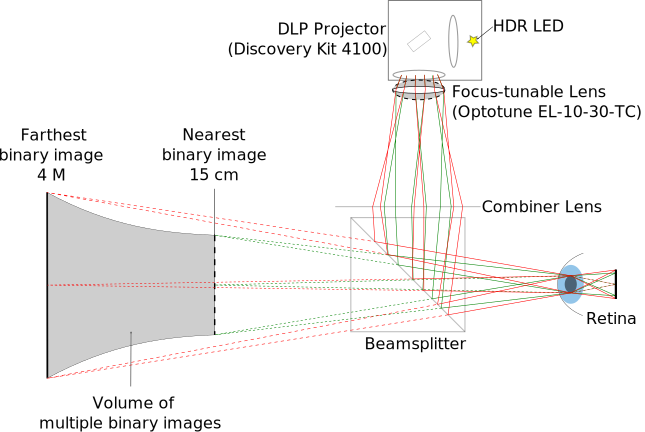
\includegraphics[width=0.99\columnwidth]{images/volumetric/proposedCandidate}
%\fbox{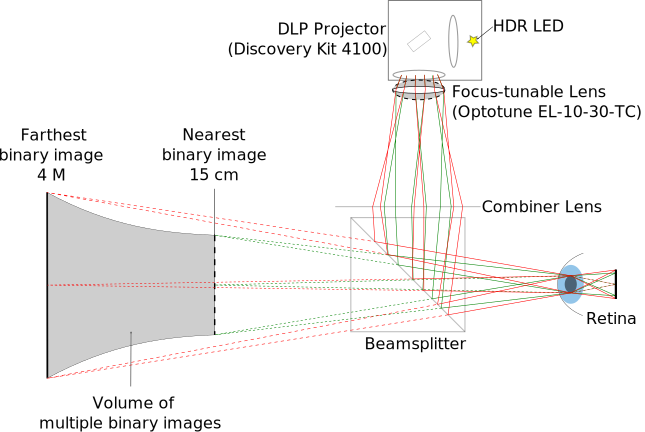
\includegraphics[width=0.46\textwidth]{images/volumetric/proposedCandidate}}
\caption[Volumetric NED: optics overview]{Figure shows an overview of the hardware and operation of our NED. The NED is composed of a high-speed HDR LED, high-speed projector, focus-tunable lens, and other common optical components. The NED's optics, rendering pipeline, and the synchronized operation of its active components (HDR LEDs, DMD, focus-tunable lens) work together to present a color volume spanning 15cm (6.7 diopters) to 4M (0.25 diopters).}
\label{fig:volumetric:proposedCandidate}
\end{figure}

\subsection{Overview of optical design} 
Our optical system is composed of multiple lenses (see Figure~\ref{fig:volumetric:unfolded}). The left diagram of Figure~\ref{fig:volumetric:unfolded} shows the image formation process for any projector. Such a projector can be converted to a near-eye display by placing an eyepiece or combiner lens just after the projected image. Since the projected image for most off-the-shelf projectors would be too large, a converging lens could be placed between the projector and the combiner lens; this helps in reducing the magnification of the projected image and in reducing the form-factor of the NED. In our NED, instead of placing a static converging lens between the projector and the combiner lens, we place a focus-tunable lens (see right diagram of Figure~\ref{fig:volumetric:unfolded}) and configure the optical power of the focus-tunable lens to sweep the real image of the DMD close to the combiner lens. To see a virtual image, the combiner lens's focal length has to be less than the distance between the lens and the real image (i.e., $f_3 < o_3(t)$).

\subsection{Modeling of optical design to derive volume geometry}
We begin with stating the Gaussian thin-lens equation
\begin{equation}
\frac{1}{f} = \frac{1}{o} + \frac{1}{i},
\label{eq:basic_optics_equation}
\end{equation}
and associated equations
\begin{equation}
i = \frac{f o}{o - f},\quad M = \frac{I}{O} = -\frac{i}{o},
\label{eq:basic_optics_equation_2}
\end{equation}
where $f$ denotes focal lens of a thin lens, $o$ denotes object distance, $i$ denotes image distance, $O$ denotes the object size, $I$ denotes image size, and $M$ denotes the magnification of the lens.

\begin{figure*}
\centering
%  \fbox{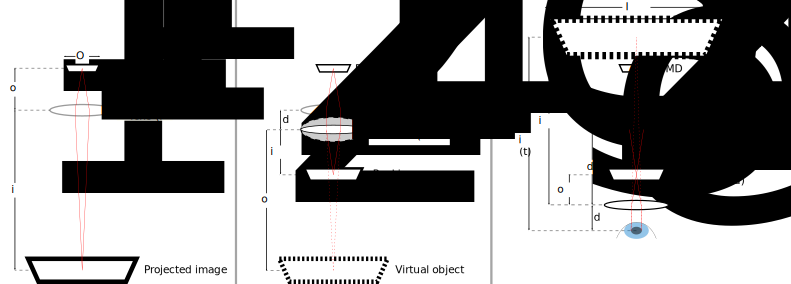
\includegraphics[width=0.46\textwidth]{images/volumetric/unfolded}}
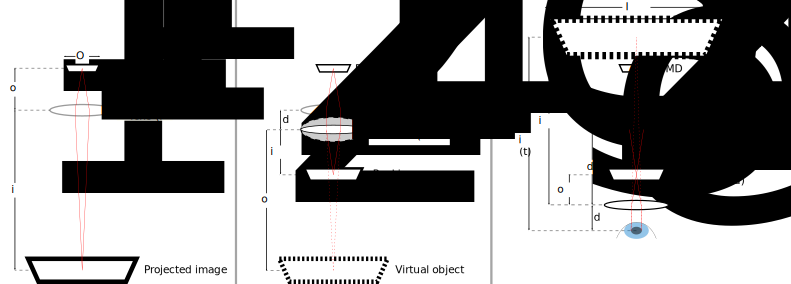
\includegraphics[width=0.95\textwidth]{images/volumetric/unfolded}
\caption[Volumetric NED: unfolded optics]{Our NED's optics can be analyzed in three stages. Figure shows the unfolded optics and ray diagram for each stage. \emph{Left: } Image formation for the DMD projector using manufacture-provided projection optics. \emph{Middle: } Adding a focus-tunable lens at the exit pupil of the DMD projector causes the real image of the DMD to be formed closer; Configuring the focus-tunable lens power to continuously oscillate causes the real image of the DMD to also oscillate. \emph{Right: } A combiner lens finally creates a virtual image of the DMD that can be seen by the eye.}
\label{fig:volumetric:unfolded}
\end{figure*}


\begin{figure}[tb!]
\centering
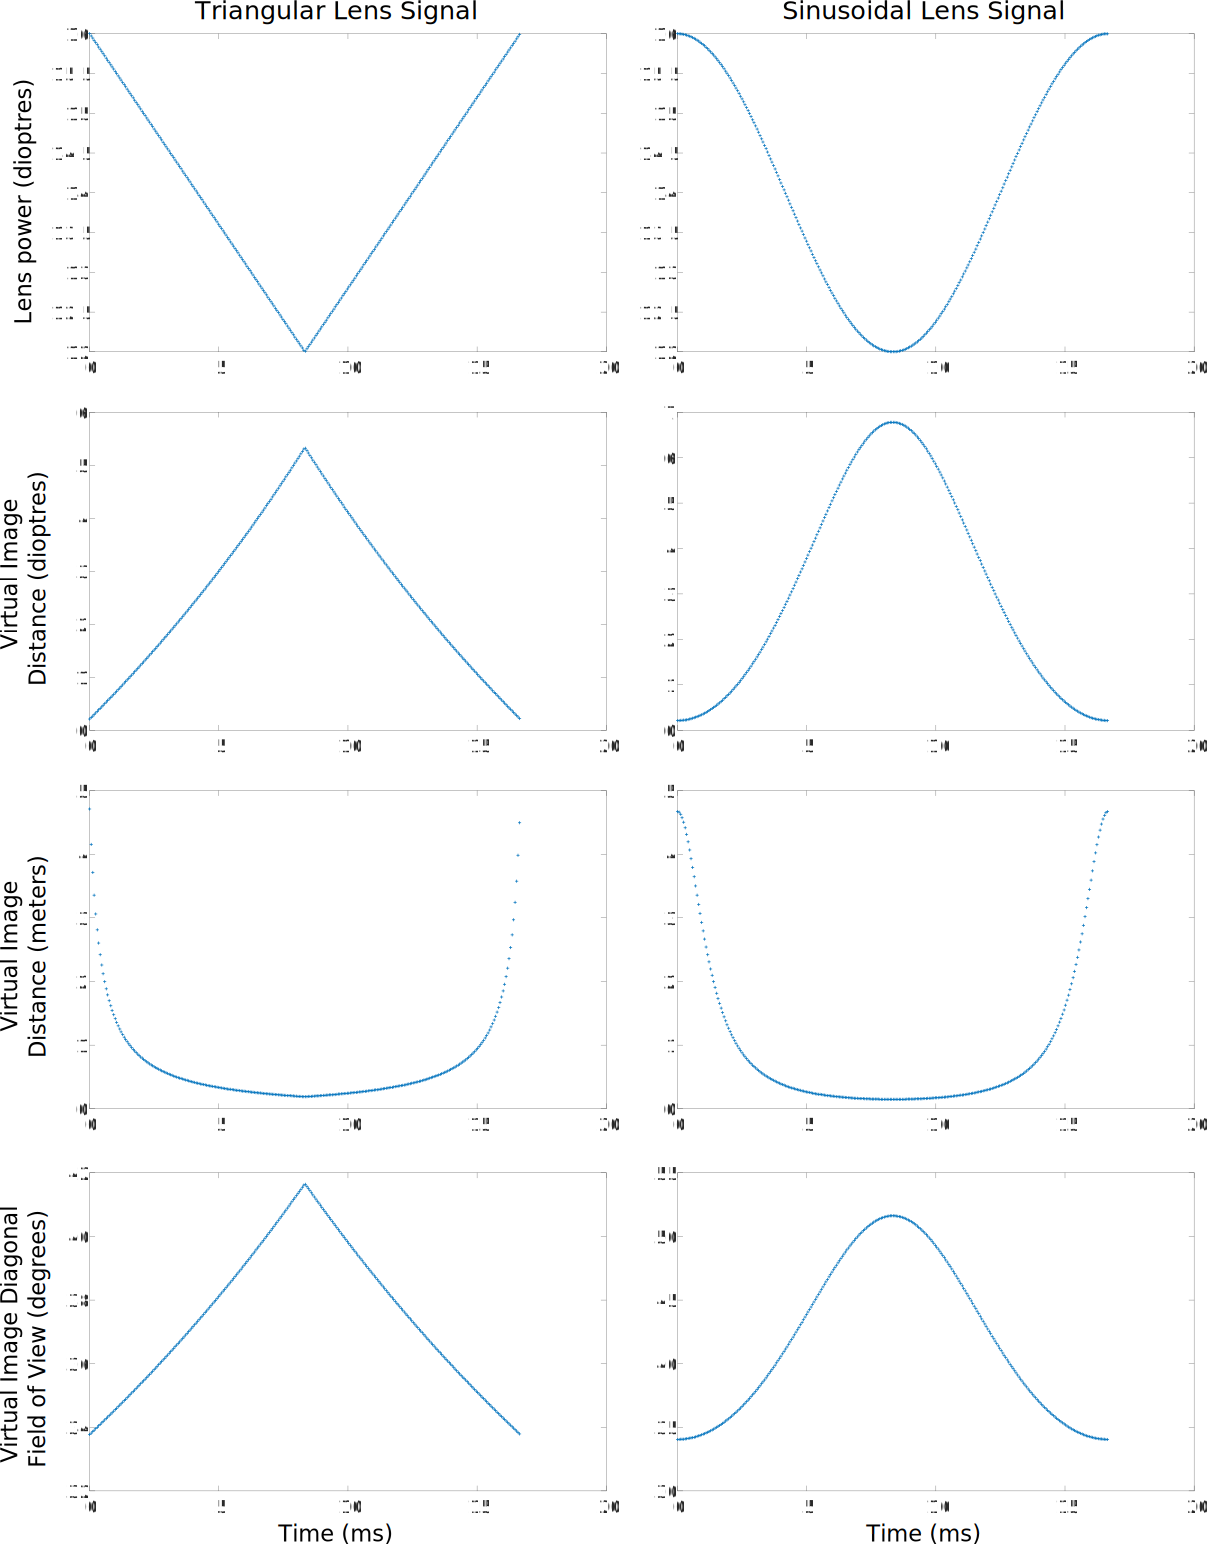
\includegraphics[width=0.9\textwidth]{images/volumetric/graphs}
\caption[Volumetric NED: graphs modelling display's depth plane distribution and FoV]{Graphs modeling the depth distribution and FoV of the displayed single-color binary images that compose the volume formed by synchronizing the DMD projector and a continuously oscillating focus-tunable lens. The oscillating lens's optical power can follow a triangular waveform \emph{(Left column)} or a sinusoidal waveform \emph{(Right column)}. Data presented in these graphs are used in the rendering pipeline to convert 3-D scene information to multiple single-color binary images that are displayed by the NED. Equations used to generate these graphs are described in Section~\ref{sec:volumetric:Optical_design}.}
\label{fig:volumetric:graphs}
\end{figure}




Due to the presence of multiple lenses in the optical stack (see Figure~\ref{fig:volumetric:unfolded}), we analyze the image formation of each lens separately and consider the image formed by each lens as the object for the next lens. This gives the following geometric relations:
\begin{equation}
o_2 = i_1-d_1, \quad o_3(t) = d_2 - i_2(t), \quad i_e(t) = i_3(t) + d_e.
\label{eq:geometric_relations}
\end{equation}

The relationship between the distance from the DMD to the projection lens ($o_1$), focal length of the projection lens $f_1$, and the projected image distance ($i_1$) is given by
\begin{equation}
i_1 = \frac{f_1 o_1}{o_1 - f_1}.
\label{eq:img1}
\end{equation}

The relationship between the object distance $o_2 = i_1 - d_1$, focal length ($f_2(t)$), and image distance ($i_2(t)$) for the focus-tunable lens is given by
\begin{equation}
i_2(t) = \frac{f_2(t) o_2}{o_2 - f_2(t)} = \frac{f_2(t) (i_1 - d_1)}{(i_1 - d_1) - f_2(t)}.
\label{eq:img2}
\end{equation}

The optical power of the focus-tunable lens ($f_2(t)$) can be configured to maintain a constant value or follow a time-varying square, triangular, or sinusoidal waveform. Other waveforms may be possible with custom electronics, but for this chapter, we analyze only the triangular and sinusoidal waveforms of lens power.

To define optical power of the focus-tunable lens as a function of time, we define some standard parameters for time-varying signals: \emph{DC bias}, \emph{amplitude}, and \emph{half-time period}. Let the DC bias, which is the average value of the signal over one full-time period be denoted by $D$. Let the amplitude, which is half of the peak-to-peak value, be denoted by $A$. Note that each cycle of the lens is the frametime of the NED. Hence, the frequency of the lens is equal to the refresh rate of the NED ($f_{\text{NED}}$). Let $a$ denote half a time period ($a = \frac{1}{2f_{\text{NED}}}$). The optical power of the focus-tunable lens, when following a triangular waveform, can be modeled as
\begin{equation}
f_2(t) = D - A\left(\frac{1}{2} - \left|\frac{t - a}{a}\right|\right),
\label{eq:general_triangular}
\end{equation}

and when following a sinusoidal waveform, it can be modeled as
\begin{equation}
f_2(t) = D + A\text{sin}(2\pi f_{\text{NED}} t).
\label{eq:general_sinusoidal}
\end{equation}

And finally, the relationship between the object distance ($o_3(t)$), focal length ($f_3$), and image distance ($i_3(t)$) for the combiner lens is given by
\begin{equation}
i_3(t) = \frac{f_3 o_3(t)}{o_3(t) - f_3} = \frac{f_3(i_2(t) + d_2)}{(i_2(t) + d_2) - f_3}.
\label{eq:img3}
\end{equation}

The above equations~\eqref{eq:geometric_relations} to \eqref{eq:img3} are sufficient to calculate the depth of each binary image plane. The FoV of the virtual binary images is found by repeated application of the magnification formula from  Equation~\eqref{eq:basic_optics_equation}:
\begin{equation}
M = M_1M_2M_3,
\label{eq:combined_magnification}
\end{equation}

\begin{equation}
I_e = MO_1,
\label{eq:virtual_image_size}
\end{equation}

\begin{equation}
\theta_{\text{FoV}} = 2\text{tan}^{-1}\left(\frac{I_e}{2i_e}\right).
\label{eq:fov}
\end{equation}

In our system, these are the values for the known quantities: $f_{\text{DMD}} = 16,800$ Hz, $f_{\text{NED}} = 60$ Hz, $f_1 = 2.96$cm, $o_1 = 3$cm, $O_1 = 1.778$cm (diagonal size of the DMD module), $d_1 = 3$cm, $f_3 = 6$cm, $d_2 = 12$cm, $d_e = 3$cm, $D = 14$, $A = 4$, and $a = 8.33$ ms. Equations~\eqref{eq:280} to \eqref{eq:fov} are evaluated with the above values to calculate the geometry of the displayed volume. The geometry of the volume is graphed in Figure~\ref{fig:volumetric:graphs}. 

The above formulation and graphs in Figure~\ref{fig:volumetric:graphs} shows only 140 unique depth planes over the time period because depth values in the first half of the time period are repeated in the second half of the time period. Our implementation is slightly different from this - we apply a small phase difference to equations~\eqref{eq:general_triangular} to \eqref{eq:general_sinusoidal} to get 280 unique depth values. 

\subsection{Sinusoidal vs. triangular waveforms}
\label{sec:volumetric:sinusoidal_vs_triangular}
In optical imaging systems, including the human eye, the blur of an object that is defocused is directly proportional to the difference between the actual distance of focus and the distance of the object in units of diopter. In our NED, the depth distribution of images should ideally be dioptrically equidistant from each other. From Figure~\ref{fig:volumetric:graphs}, it can be seen that the lens power following a triangular waveform results in a near-linear and equidistant distribution of virtual image planes in dioptric space. Hence, we implemented the rendering pipeline and electronic synchronization assuming that the lens sweeps a triangular waveform. However, when we used the sinusoidal waveform in place of a triangular waveform, keeping everything else such as the color decomposition, and electronic synchronization the same, we didn't notice a significant difference in the displayed volume geometry and image quality. This may be either because the difference between the triangular and sinusoidal waveforms is negligible compared to the minimum dioptric difference required to make a perceptual difference or because the lens' triangular and sinusoidal waveforms are similar, which can often happen with physical systems due to inertia/friction, etc., especially at higher frequencies.

\section{Rendering Pipeline}
\label{sec:volumetric:rendering_pipeline}
In this section, we first discuss the rendering pipelines of previous DMD-based NEDs, then describe our full rendering pipeline from graphics primitives to single-color binary images, and finally discuss the benefits and limitations of our rendering pipeline.

\subsection{Rendering pipeline for previous DMD-based NEDs}
\label{sec:volumetric:previous_rendering_pipeline}


% Main constraint in binary multifocal displays
% Previous rendering pipelines
\subsubsection{Low latency and HDR NEDs}
Most display technologies that employ a DMD also use a constant intensity or bivalent illumination source and use pulse train modulation to create grayscale or color imagery~\cite{Lincoln2016motion}. Recently, Lincoln et al.\cite{Lincoln2017scene} demonstrated a DMD-based display system which used a controllable high-speed HDR illuminator. They demonstrated that the intensity and color of the illumination could be changed over a wide range on a per-binary frame basis. They also proposed a new color to binary decomposition method, which they call \emph{Direct Digital Synthesis (DDS)}. Let $d$ be the desired color intensity value, $g$ be the generated color intensity value, and $s$ be the step index of the binary representation of the value of $d$. Then, DDS decomposition from color to binary values can be represented per color channel as shown below: 

\begin{equation}
g = \sum_{s = 0}^{n-1} \left(2^s \times \text{bit}(d,s)\right).
\end{equation}

\subsubsection{Multifocal plane NEDs}
Previous DMD-based multi-focal plane displays~\cite{Hu2014design,Hu2015Design} decomposed a 3-D scene to a stack of \emph{color images} fixed at the various depths. In these approaches, the focus-tunable lens or deformable membrane mirrors would step through a set of focal lengths, and at each focal length, \emph{after the lens stabilizes}, a series of binary images was displayed by one of the classical pulse train modulation schemes to generate color imagery. For such color image plane based approaches, we provide equations below for the relationship between the DMD's framerate ($f_{\text{DMD}}$), number of focal planes ($N_{\text{planes}}$), framerate of the NED ($f_{\text{NED}}$), and the color depth per color channel ($N_{\text{gray}}$). Up to some extent, a multifocal NED with a larger number of $N_{\text{planes}}$ can present better imagery because the scene decomposition algorithms of depth fused multifocal displays trade-off the spatial frequency of the fused image and the focal plane separation~\cite{Hu2014design,Hua2017Enabling}. 

In case of classical pulse train modulation schemes, the number of focal planes is given by
\begin{equation}
N_{\text{planes}} = \frac{f_{\text{DMD}}}{3 f_{\text{NED}} (2^{N_{\text{gray}}}-1)}.
\end{equation}

Using DDS decomposition, $N_{\text{planes}}$ can be increased significantly as shown by the following equation
\begin{equation}
N_{\text{planes}} = \frac{f_{\text{DMD}}}{3 f_{\text{NED}} N_{\text{gray}}}.
\end{equation}

A DMD-based multifocal display which decomposes 3-D scene information to color image planes which are in turn decomposed from color images to binary images based on DDS decomposition has not been demonstrated. If it were demonstrated with our hardware ($f_{\text{DMD}} = 16,800$ Hz, $N_{\text{gray}}=8$, $f_{\text{NED}}=60$ Hz), we would achieve $N_{\text{planes}}=11$ color image planes. However, we propose a further improvement below based on voxel-oriented decomposition rather than image-oriented decomposition. 

%Using any modulation scheme, for all image plane based multifocal displays, the average separation in depth between two non-coplanar pixels is $\frac{R}{N_{\text{planes}}}$ diopters where the focus range of the display is $R$ diopters.

\begin{figure}[t]
\centering
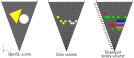
\includegraphics[width=\columnwidth]{images/volumetric/binary_decomposition}
\caption[Volumetric NED: color volume to binary volume decomposition]{Diagram shows the stages of our rendering pipeline: voxelization (see Section~\ref{sec:volumetric:Voxelization}) and binary decomposition (see Section~\ref{sec:volumetric:Decomposition}). For ease of representation, the figure depicts the rendering pipeline for a simple 2-D graphics and 6 bits-per-pixel imagery. Actual implementation uses 3-D graphics and 24 bits-per-pixel imagery. The numbers along the displayed binary volume's frustum indicate the intensity level and color of the RGB LED that illuminates the current binary image.}
%The focal planes are depicted here as equidistant from each other only for ease of representation.}
%Even though the diagram indicates the color volume and binary volume to be in a perspectively shaped volume, the computation is carried out in an orthographic (rectangular) volume. When the display presents the images, it performs an automatic inverse-perspective transformation that corrects for our computations which carried out in the rectangularly shaped volume \kishore{Shorten caption}.}
\label{fig:volumetric:binary_decomposition}
\end{figure}



\subsection{An overview of our rendering pipeline}
The pipeline currently handles only opaque polygons; transparency and other primitives are left to future work. Our rendering pipeline is composed of two steps: (1)  \emph{voxelization}, i.e., the process of converting 3-D polygonal data to a 2-D surface composed of color voxels (3-D equivalent of pixels) that best approximates 3-D polygonal data; and (2) \emph{decomposition} of the color voxels into a series of binary images and corresponding illumination values; these data are used by the display to present a series of single-color binary images to the viewer. 
%Our rendering pipeline can be understood as in three steps: (1) Using 3-D models and scene data, an OpenGL renderer generates an RGB image and a linearized depth map of the current scene at the resolution of the DMD display ($1024 \times 768$).  (2) \emph{voxelization}, i.e., the process of converting graphics primitives from their continuous geometric representations into a set of voxels (3-D equivalent of pixels) that best approximates the graphics primitives; and (3) \emph{decomposition} of the color voxels into a series of binary images and corresponding illumination values; these data are used by the display to present series of binary images to the viewer. \kishore{Mention color}

%We then calculate the color volume by back-projecting the RGB and depth data orthographically. We decompose the color volume to a binary volume on a per-color-voxel basis where the binary voxels corresponding to a color voxel are distributed parallel to the optical axis of the display. The binary images are then displayed on our prototype display, which automatically does a near-inverse perspective projection of the calculated binary images. This is then integrated in the eye or camera to perceive a color volume. 

\subsection{Voxelization: Graphics primitives to 2-D surface}
\label{sec:volumetric:Voxelization}
Using 3-D models and scene data, an OpenGL renderer generates an RGB image and a linearized 16-bit depth map of the current scene at the resolution of the DMD display ($1024 \times 768$). The 16-bit values of the depth map are remapped to the 280 depth values of the focal planes supported by our optical design. This results in a 2-D surface, composed of color voxels, in a $1024 \times 768 \times 280$ volume.

\subsection{Binary Decomposition: Color voxels to binary images}
\label{sec:volumetric:fixed_pipeline}

Our key observation is that the binary representation of a color voxel need not start or end at one of the modulo $3 \times (2^{N_{\text{gray}}} - 1)$ planes as proposed by earlier binary multifocal displays. It need not start or end at one of the modulo $3 \times N_{\text{gray}}$ also, as would be the case for a multifocal NED which displays color image planes using DDS decomposition. Instead, the decomposition of a color voxel to binary voxel can begin and end at arbitrary depths. 

When converting from color volume data to binary images, the intensity and color of each color voxel tell us the binary pattern that represents it, and the depth of the color voxels tells us the center around which the binary pattern should be distributed. The binary voxels that encode the color voxel are distributed along the perspective projection lines that pass through the color voxel's location and the distribution is centered around the color voxel's location. Figure~\ref{fig:volumetric:binary_decomposition} provides a visualization of our rendering pipeline. For ease of representation, Figure~\ref{fig:volumetric:binary_decomposition} depicts the rendering pipeline for equidistant focal planes and for 2-D graphics generating 6 bits-per-pixel imagery. Our implementation handles 24-bits-per-pixel color imagery.


If this decomposition was implemented in an acyclic manner, the number of unique color voxel depths would be $N_b - (3 \times N_{\text{gray}}) + 1$, which is $257$ planes in our case. However, we could implement this decomposition in a cyclic manner, and in this case, the number of unique color voxel depths would be equal to $N_b$, which is 280 in our case. 

Even though we depict in Figure~\ref{fig:volumetric:binary_decomposition} that the decomposition happens in a perspectively shaped volume, it can be implemented as a decomposition on a rectangularly shaped volume. This is indeed the case in our implementation. This is not an issue because when the NED displays the single-color binary images, it does a near-inverse perspective transformation. 

\subsection{Display: Binary images to Retinal image}
The binary images generated are displayed on a DMD in sync with a focus-tunable lens sweeping a sinusoidal or triangular waveform for the optical power of the lens. The single-color binary images displayed by the NED are integrated by the eye to see a color volume. Displaying the binary images in our prototype display is a near inverse-perspective transformation. It is not a perfect inverse-perspective transformation due to the slight change in FoV of images seen over the cycle of the lens (see Figure~\ref{fig:volumetric:graphs}). This near inverse-perspective transformation allows us to perform the transformation of RGB and depth images to color voxels, and the transformation of color voxels to binary voxels in an orthographic space. 

\subsection{Limitations}
\subsubsection{Depth and Spatial resolution}
Conceptually, the minimum non-zero separation in depth between two voxels in our display is $1$ depth plane which averages to $\frac{\text{6.7 diopters}}{\text{280 focal planes}}=\text{0.024 diopters}$. However, because the binary voxels are spread across multiple binary image planes, we should expect to see a blur for the color voxel along the optical axis which could lead to a loss in the depth resolution of the NED. Since each color voxel is represented by multiple binary voxels and the brighter binary voxels are going to be perceived more strongly, we calculate the depth blur as the \emph{weighted} standard deviation of sorted depth values for a moving window of length $3 \times N_{\text{gray}}=24$; this is graphed in the top row of Figure~\ref{fig:volumetric:blur_graphs}. 

Similarly, due to the slightly changing FoV of binary images across the lens cycle (shown in Figure~\ref{fig:volumetric:graphs}), we should expect to see a blur perpendicular to the optical axis which could lead to a loss in the spatial resolution of the NED. This blur is minimum for pixels close to the optical axis and maximum for pixels at the periphery. The maximum angular blur perpendicular to the optical axis is calculated as the standard deviation of FoV values for a moving window of length $3 \times N_{\text{gray}}=24$; this is graphed in the bottom row of Figure~\ref{fig:volumetric:blur_graphs}.

The blur perpendicular to the optical axis can be reduced by performing a calibration to determine the actual FoV of each binary image plane and modifying the color to binary decomposition algorithm to take into account the deformed volume geometry. We did not perform such a calibration process for this chapter. The blur along the optical axis, however, is more fundamental to the display technology. It could be reduced by advanced color volume to binary volume decomposition schemes. 

Previous works have suggested slightly different values for the focal plane separation required for a good multifocal display. Rolland et al.~\cite{Rolland1999dynamic} suggest 0.143 diopters, Akeley et al.~\cite{Akeley2004} design their prototype with image spacings of 0.67 diopters, Liu et al.~\cite{Liu2010systematic} and Watt et al.~\cite{Watt2012Real} suggest 0.6 diopters, and MacKenzie et al.~\cite{MacKenzie2010Accommodation} suggest 1 diopter. As shown in Figure~\ref{fig:volumetric:blur_graphs}, our display has a maximum depth-blur of 0.3 diopters and an average depth-blur of 0.167 diopters. 

\begin{figure}[tb!]
\centering
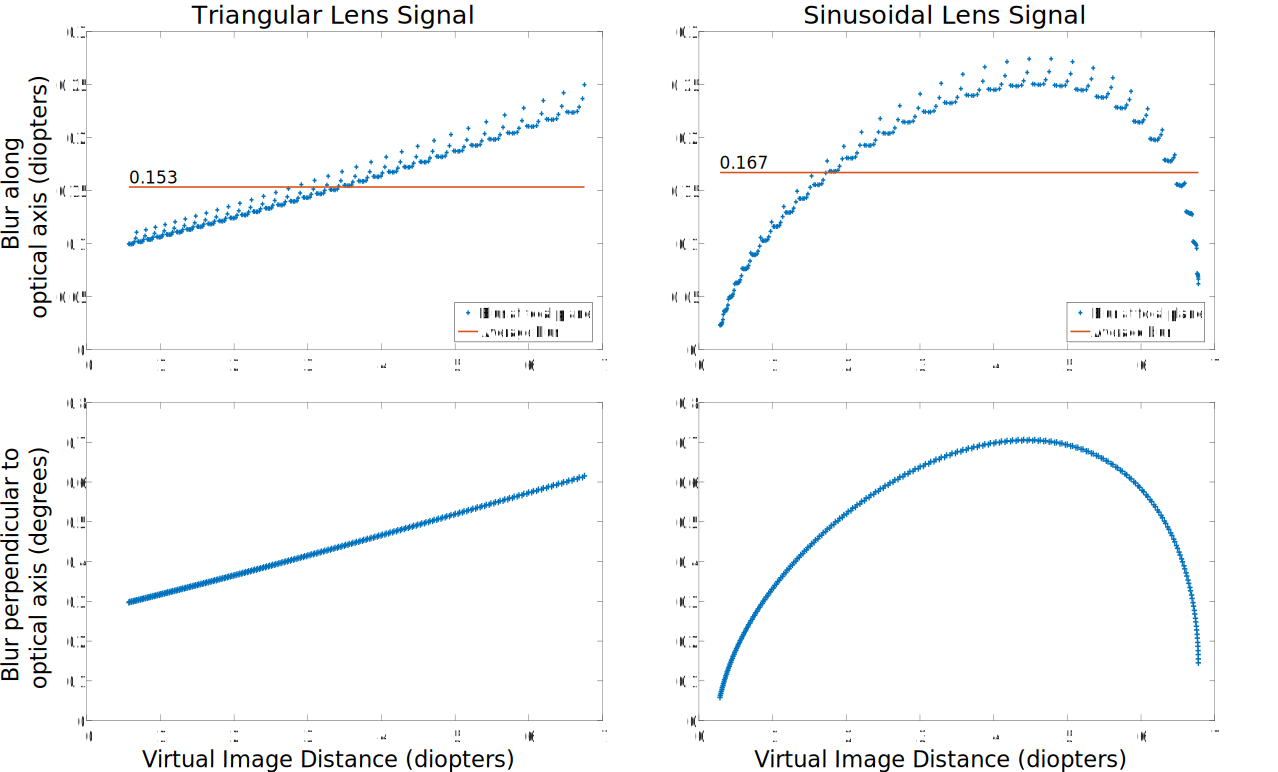
\includegraphics[width=\columnwidth]{images/volumetric/blur_graphs}
\caption[Volumetric NED: Longitudinal and lateral blur of voxels at each depth plane]{\emph{Top row: }Graphs indicate the depth blur for a color voxel at each depth plane and the average depth blur for color voxels of all depth planes. The depth blur arises because the rendering pipeline decomposes each color voxel to multiple single-color binary voxels, which are spread along the perspective projection lines. \emph{Bottom row: } The optics of our NED cause the FoV of the virtual image to slightly change over the lens cycle; this changing FoV is graphed. This creates a blur perpendicular to the optical axis leading to a loss in spatial resolution.}
\label{fig:volumetric:blur_graphs}
\end{figure}
    
    


\subsubsection{Voxel-fighting in a dynamic display implementation}
Here we discuss a minor limitation in extending our proposed offline rendering pipeline to a dynamic display. Observe that to decompose a single color voxel for a 24 bits-per-pixel image, we require 24 binary voxels. In the case of a static display and a cyclic implementation of our decomposition algorithm, this means that a color voxel at, say, the 280th focal plane would be decomposed into binary voxels that range from binary image indices 268 to 12. However, in a dynamic display case, we run into the issue that a new frame is received for each display cycle. 

If the incoming frame information completely replaces the previous frame information, there could be a loss of brightness and bit-depth for the color voxels in the last few focal planes. Alternatively, if we design the NED to start displaying the new frame information only after it finishes displaying the previous frame information, the DMD display's cycle would quickly fall out-of-sync with the lens cycle. With a modified rendering pipeline, for which the framerate of the NED is slightly lower than the frequency of the focus-tunable lens, and very good synchronization of the lens and the DMD, this would not be an issue. Alternatively, we could carry over the information of the last few focal planes of the previous frame to the new frame while giving priority/preference to the new frame's information. 

